\documentclass[tikz]{standalone}

\usepackage{amsmath}
\usepackage{tikz}
\usetikzlibrary{arrows}
\usetikzlibrary{calc}
\usepackage{ifthen}

\newcommand{\vct}[1]{\boldsymbol{#1}}
\newcommand{\pd}[2]{\frac{\partial #1}{\partial #2}}

\tikzstyle{fprop} = [draw,fill=blue!20,minimum size=2em,align=center]
\tikzstyle{bprop} = [draw,fill=red!20,minimum size=2em,align=center]

\begin{document}

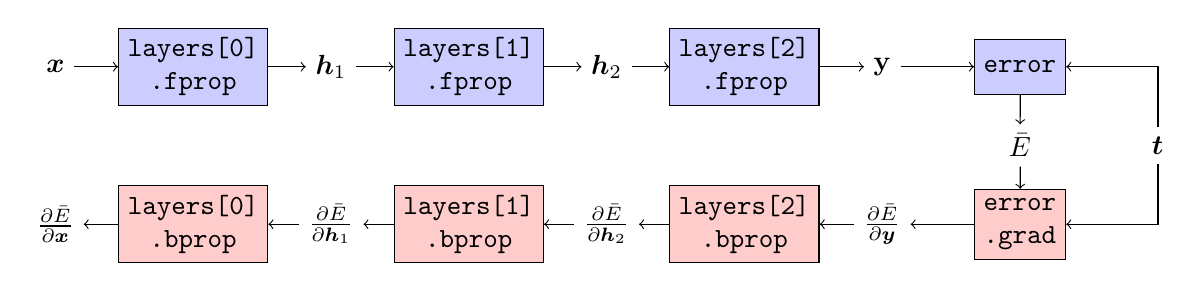
\begin{tikzpicture}[xscale=1.75] %
    % define number of layers
    \def\nl{2};
    % model input
    \node at (0, 0) (input) {$\vct{x}$};
    % draw fprop through model layers
    \foreach \l in {0,...,\nl} {
        \node[fprop] at (2 * \l + 1, 0) (fprop\l) {\texttt{layers[\l]} \\ \texttt{.fprop}};
        \ifthenelse{\l > 0}{
            \node at (2 * \l, 0) (hidden\l) {$\vct{h}_\l$};
            \draw[->] (hidden\l) -- (fprop\l);
            \draw[->] let \n1={\l - 1} in (fprop\n1) -- (hidden\l);
        }{
            \draw[->] (input) -- (fprop\l);
        }
    }
    % model output
    \node at (2 * \nl + 2, 0) (output) {$\mathbf{y}$};
    % error function
    \node[fprop] at (2 * \nl + 3, 0) (errorfunc) {\texttt{error}};
    % error value
    \node at (2 * \nl + 3, -1) (error) {$\bar{E}$};
    % targets
    \node at (2 * \nl + 4, -1) (tgt) {$\vct{t}$};
    % error gradient
    \node[bprop] at (2 * \nl + 3, -2) (errorgrad) {\texttt{error} \\ \texttt{.grad}};
    % gradient wrt outputs
    \node at (2 * \nl + 2, -2) (gradoutput) {$\pd{\bar{E}}{\vct{y}}$};
    \draw[->] (fprop\nl) -- (output);
    \draw[->] (output) -- (errorfunc);
    \draw[->] (errorfunc) -- (error);
    \draw[->] (error) -- (errorgrad);
    \draw[->] (errorgrad) -- (gradoutput);
    \draw[->] (tgt) |- (errorfunc);
    \draw[->] (tgt) |- (errorgrad);
    \foreach \l in {0,...,\nl} {
        \node[bprop] at (2 * \l + 1, -2) (bprop\l) {\texttt{layers[\l]} \\ \texttt{.bprop}};
        \ifthenelse{\l > 0}{
            \node at (2 * \l, -2) (grad\l) {$\pd{\bar{E}}{\vct{h}_\l}$};
            \draw[<-] (grad\l) -- (bprop\l);
            \draw[<-] let \n1={\l - 1} in (bprop\n1) -- (grad\l);
        }{}
    }
    \node at (0, -2) (gradinput) {$\pd{\bar{E}}{\vct{x}}$};
    \draw[->] (bprop0) -- (gradinput);
    \draw[->] (gradoutput) -- (bprop\nl);
\end{tikzpicture}

\end{document}